We used an actor-critic algorithm as approximator. The applied optimization algorithm is Adam.
The actor network produces actions learned via the Proximal Policy Optimization (PPO). Both actor and critic are multilayer perceptrons (MLP), see Table \ref{table:network} and Figure \ref{fig:actor} for details on their architectures.
\begin{table*}[t]
\centering
\caption{Network architecture.}
\begin{tabular}{c|c|c|c|c|c|c|c} 
 \hline 
 Network & Type & Input & Hidden Layer & Activation & Last Layer & Output & Output Size \\ [0.1ex] 
 \hline
 \hline
 \multirow{2}*{actor} & \multirow{2}*{MLP} & \multirow{2}*{observation} & \multirow{2}*{2x128} & \multirow{2}*{tanh} & 1x128 & action mean & 2 \\ [0.1ex]
    & & & & & 1x128 & action variance & 2 \\ [0.1ex]
 \hline
 critic & MLP & observation & 2x128 & tanh & 1x128 & value & 1 \\ [0.1ex] 
 \hline
\end{tabular}
\label{table:network}
\end{table*}

The chosen observation space and reward function are based on the suggestions of Penicka et al. \cite{Penicka_2022}.
The observations consist of two parts: the VTOL drone's state (world position, body orientation, as well as the translational and rotational velocities) and the relative path to the next two waypoints. 
The VTOL drone model provided by Flyonic \cite{flyonic} allows four possible actions: 
regulating thrusts of two propellers and adjusting angles of two flaps. 
% setting the rotation speed of the two propellers individually, as well as adjusting the angle of the two flaps the drone possesses.
In Figure \ref{fig:actor} both observation and action space are illustrated.
\begin{figure}[ht]
    \centering
    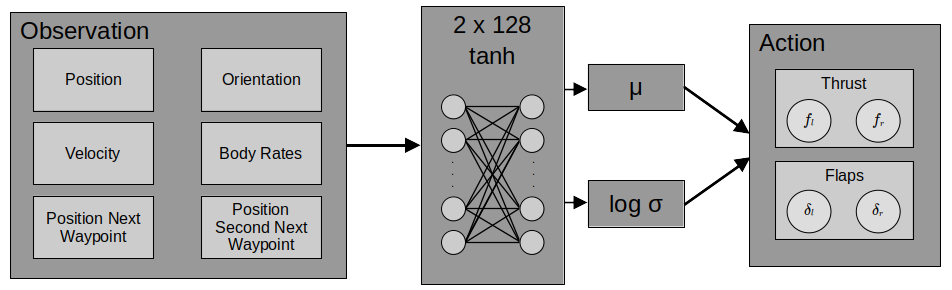
\includegraphics[width=8cm]{images/actor_short.png}
    \caption{Illustration of the actor network with the used observation and action space.}
    \label{fig:actor}
\end{figure}

The reward function consist of five parts: encouraging progression along the trajectory (connected lines between $n$ waypoints $g_1,...,g_n$) in every time step, rewarding the overall reached distance along the trajectory, rewarding reached waypoints, penalizing high body rates $\omega$ and penalizing inactivity. To calculate the progress at position $p$ we define the closest point on the trajectory as $\psi(p)$ and its corresponding line segment index as $l(p)$. See an example illustration in Figure \ref{fig:trajectory}.
\begin{figure}[b]
    \centering
    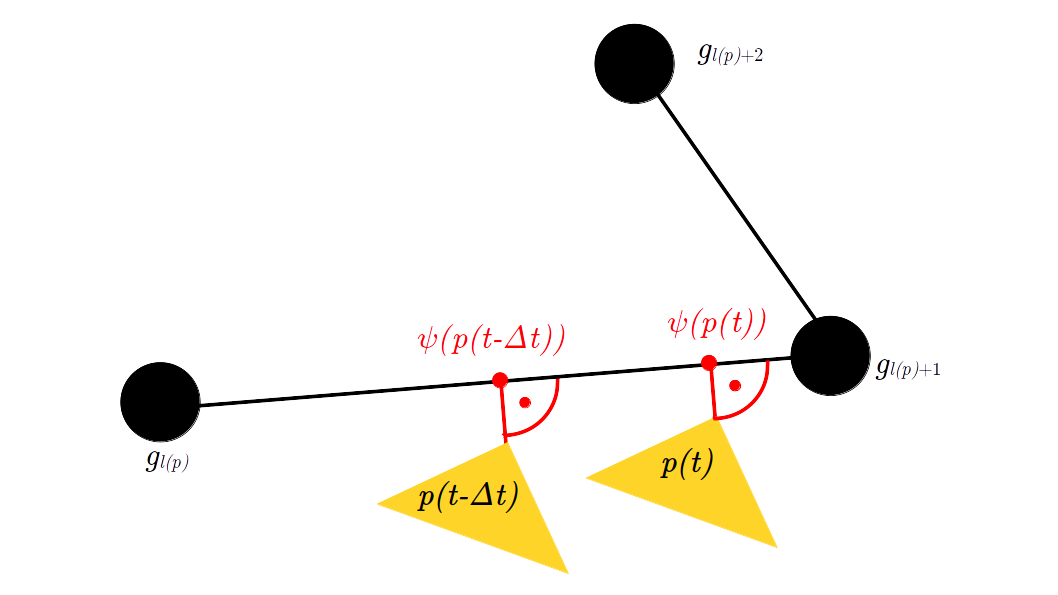
\includegraphics[width=6.5cm]{images/trajectory.png}
    \caption{Illustration of trajectory with three waypoints. The nearest point $\psi(p)$ on trajectory from drone at position $p$ and its corresponding line segment index $l(p)$ is used to calculate the progress in each time step $\Delta t$ and the reached distance.}
    \label{fig:trajectory}
\end{figure}
The total reward function $r(t)$ at time $t$ is defined as 
\begin{align*}
r(t) = k_p r_p(t) + k_s s(p(t)) + k_{wp} r_{wp} + k_\omega \|\omega\| - fall,
\end{align*}
with the reached distance along the trajectory $s(p(t))$ and the progress reward at each time step $r_p(t)$ being defined as
\begin{align*}
    &s(p) = \sum_{i=1}^{l(p) - 1} \| g_{i+1} - g_i \| + \|\psi(p) - g_{l(p)}\|, \\
    &r_p(t) = s(p(t))-s(p(t- \Delta t)).
\end{align*}
The reached distance $s(p(t))$ is part of the reward function to counteract possible singularities due to sharp corners of the trajectory and the minimum distance projection. The reward $r_{wp}$ was payed, if the drone reached a waypoint within a distance $d_{wp}$ smaller than a tolerance $r_{tol}$ for the first time. The penalty term $fall$ was only subtracted if the drone fell under $-1$m due to inactivity. The contribution of each reward part is scaled by the hyperparameters $k_p$, $k_s$, $k_{wp}$ and $k_{\omega}$.

We initially focused on learning a slow and stable flying policy, henceforth referred to as \textit{slow learning phase}. Therefore, the hyperparameters $k_s$ and $k_p$ were scaled by a factor $s_m$ that encouraged translation velocities between $v_{min}$ and $v_{max}$. This factor also motivates the drone to stay within a distance of $d_{max}$ to the trajectory. The scaling factor $s_m$ is calculated as
\begin{align*}
 & s_m = s_{v} \cdot s_{gd}, \\
 & s_{v} = \min(1, 10^{v_{max}-||v||}) \cdot \min(1, 10^{||v||-v_{min}}), \\
 & s_{gd} = \min(1,e^{ - \|p - \psi(p) \| + d_{max}}).
\end{align*}
For our training process the values in Table \ref{table:parameters} were used.
\begin{table}[h]
\centering
\caption{Parameters of the algorithm.}
\begin{tabular}{c c|c c} 
 \hline 
 Variable & Value & Variable & Value \\ [0.1ex] 
 \hline
 \hline
 $v_{min}$ [m/s] & $1.0$ & $v_{max}$ [m/s] & $3.0 $ \\ [0.2ex]
 $\Delta t$ [s] & $0.025$ & $fall$ [-] & 1 \\ [0.2ex]
 $n$ & 4 & $k_{wp}$ [-] & $10.0 n$ \\ [0.2ex]
 $r_{tol}$ [m] & 0.5& $r_{wp}$ & $\exp(d_{wp}/r_{tol})$ \\ [0.2ex]
 $k_p$ [-] & $5.0$ & $k_\omega$ [-] & 0.01 \\ [0.2ex] 
 $k_s$ [-] & $\frac{2v_{max}\Delta t}{\sum_{i=1}^{n-1} \|g_{i+1} -g_i\|}$ & $d_{max}$ [m] & 0.2 \\[2ex] 
 \hline
\end{tabular}
\label{table:parameters}
\end{table}